\documentclass[xcolor=table]{beamer}
\usepackage{lmodern}
%\usepackage[normalem]{ulem}
\usepackage{ marvosym }
\usepackage[export]{adjustbox}
\usepackage{mathtools,calc}
\newcommand\Fontvi{\fontsize{22}{23.2}\selectfont}
\newcommand\strikeout[2][]{%
 \begin{tabular}[b]{@{}c@{}}
    \makebox(0,0)[cb]{\textcolor{blue}{#1}} \\[-0.2\normalbaselineskip]
     \rlap{\color{red}\rule[0.5ex]{\widthof{#2}}{0.5pt}}#2
 \end{tabular}}

\newcommand<>\mathalt[2]{%
  \alt#3{\mathmakebox[\widthof{$#2$}]{#1}}{#2}%
}
\newcommand{\underbracedmatrix}[2]{%
  \left(\;
  \smash[b]{\underbrace{
    \begin{matrix}#1\end{matrix}
  }_{#2}}
  \;\right)
  \vphantom{\underbrace{\begin{matrix}#1\end{matrix}}_{#2}}
}
\usepackage{colortbl}
\usepackage{minted}
\usepackage{booktabs}
%\usepackage{xcolor}
%\usepackage[usenames, dvipsnames]{color}
\definecolor{red}{rgb}{0.894, 0.101, 0.109} 
\definecolor{Gray}{gray}{0.85}
\newcolumntype{a}{>{\columncolor{Gray}}c}
\definecolor{green}{rgb}{0.1054, 0.6171, 0.4648}
\definecolor{orange}{rgb}{0.8476, 0.3711, 0.0078}
\definecolor{violet}{rgb}{0.9023, 0.1602, 0.5391}
\usepackage[doi=false, backref=true, url=false, isbn=false, backend=biber,
                        citestyle=authoryear]{biblatex}
\usepackage{tabu}
\newcommand{\blue}{\textcolor{blue}}
\newcommand{\red}{\textcolor{red}}
\newcommand{\green}{\textcolor{green}}
\newcommand{\organge}{\textcolor{orange}}
\newcommand{\violet}{\textcolor{violet}}
% Just for demo

\AtBeginSection[]{
  \begin{frame}
  \vfill
  \centering
  \begin{beamercolorbox}[sep=8pt,center,shadow=true,rounded=true]{title}
    \usebeamerfont{title}\insertsectionhead\par%
  \end{beamercolorbox}
  \vfill
  \end{frame}
}
\usepackage{mathtools}
\newtheorem{prop}{Proposition}
\newtheorem{hypothesis}{Hypothesis}
\usepackage{amsmath}
\usepackage{multirow}
\usepackage{makecell} % to make linebreaks in table
\renewcommand\theadalign{bc}
\renewcommand\theadfont{\bfseries}
\renewcommand\theadgape{\Gape[4pt]}
\renewcommand\cellgape{\Gape[4pt]}
\usepackage{hhline}
\usepackage{geometry}
\usepackage{booktabs}
\usepackage[]{hyperref}%
\hypersetup{colorlinks, linkcolor={blue}, citecolor={blue}, urlcolor={red}}
\usepackage{graphicx}

\DeclareMathOperator*{\argmax}{\arg\!\max}
\DeclareMathOperator{\E}{\mathbb{E}}
\addbibresource[]{library.bib}
\usepackage[utf8]{inputenc}
\usepackage[T1]{fontenc}
\setbeamertemplate{caption}{\raggedright\insertcaption\par}
\usetheme{default}
\usepackage[flushleft]{threeparttable}
\usepackage{booktabs,caption,fixltx2e}
\usepackage{ragged2e}
\usepackage{appendixnumberbeamer}
\makeatletter
\usefonttheme{professionalfonts}
\usefonttheme{serif}
\setbeamertemplate{navigation symbols}{}%remove navigation symbols
\setbeamertemplate{footline}
{
  \leavevmode%
  \hbox{%
  \begin{beamercolorbox}[wd=.333333\paperwidth,ht=2.25ex,dp=1ex,center]{author in head/foot}%
    \usebeamerfont{author in head/foot}\insertsection\
  \end{beamercolorbox}%
  \begin{beamercolorbox}[wd=.333333\paperwidth,ht=2.25ex,dp=1ex,center]{title in head/foot}%
    \usebeamerfont{title in head/foot}\insertsubsection\
  \end{beamercolorbox}%
  \begin{beamercolorbox}[wd=.333333\paperwidth,ht=2.25ex,dp=1ex,right]{date in head/foot}%
    %\usebeamerfont{date in head/foot}\insertshortdate{}\hspace*{2em} % hide %date
    %\insertframenumber{} / \inserttotalframenumber\hspace*{2ex} 
  \end{beamercolorbox}}%
  \vskip0pt%
}
\makeatother
%\setbeamertemplate{footline}[frame number]{}


\usepackage{listings}
\lstset{
    tabsize=4,
    showstringspaces=false,
    numbers=left,
    commentstyle=\color{green},
    keywordstyle=\color{blue},
    stringstyle=\color{red}
}


 %----------------------------------------------------------------------------------------
% %	TITLE PAGE
% %----------------------------------------------------------------------------------------
\renewcommand*{\thefootnote}{\fnsymbol{footnote}}
\title[]{Mergesort with CUDA}
\date{\parbox{\linewidth}{\centering%
  25.02.2020\endgraf\bigskip
  Fork on Github:\\
  \blue{https://github.com/FabianSchuetze/mergesort}
  }}
%\date{25.02.2020} % Date, can be changed to a custom date
%\author{Fabian Schuetze, EUI}
\addtobeamertemplate{block begin}{}{\justifying}  %new code
\setbeamertemplate{itemize items}[circle]

\usepackage{tikz, enumitem}
\usetikzlibrary{positioning}% for positioning of nodes
\usetikzlibrary{decorations.pathreplacing,positioning, arrows.meta}
\newcommand{\ImageWidth}{11cm}


\begin{document}
\author{Fabian Schuetze}

\begin{frame}
\titlepage
\end{frame}

\begin{frame}
\frametitle{GPU: fast, cheap, and approachable}
    \red{Fast:}
\begin{figure}[ht]
   \centering
   \includegraphics[scale=0.25]{flops.png}
\end{figure}
    \red{Cheap:} CPU: $\$400$, GPU: $\$200$\\
    \red{Approachable:} CUDA: C++ Syntax, called from C and C++
\end{frame}

\begin{frame}
\tableofcontents
\end{frame}


\section{Intro I: Simple Program}

\begin{frame}[fragile]
\frametitle{A Simple Cuda Program}
\begin{overlayarea}{\textwidth}{7.1cm}
%\only<1->{
\begin{onlyenv}<1->
\green{1: Call Cuda Program from C and C++:}
\begin{minted}[linenos=true]{cpp}
dim3 Grid(2)
dim3 Block(4)
square<<<Grid, Block>>>(...)
\end{minted}
\end{onlyenv}
%}
\begin{onlyenv}<2->
    \green{2: Blocks \& Grid spawn Threads:}
\begin{figure}
    \centering
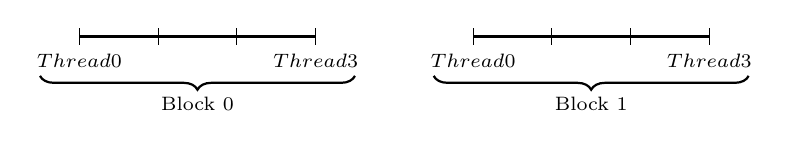
\begin{tikzpicture}
% draw horizontal line
\draw[thick,- ] (0,0) -- (3,0) node[font=\scriptsize,below left=3pt and
        -5pt]{};
\draw[thick,- ] (5,0) -- (8,0) node[font=\scriptsize,below left=3pt and
        -5pt]{};


% draw vertical lines
\foreach \x in {0,1,...,3}
\draw (\x cm,3pt) -- (\x cm,-3pt);

\foreach \x in {5,6,...,8}
\draw (\x cm,3pt) -- (\x cm,-3pt);

\foreach \x/\descr in {0/Thread 0,3/Thread 3}
\node[font=\scriptsize, text height=1.75ex,
text depth=.5ex] at (\x,-.3) {$\descr$};

\foreach \x/\descr in {5/Thread 0,8/Thread 3}
\node[font=\scriptsize, text height=1.75ex,
text depth=.5ex] at (\x,-.3) {$\descr$};

\draw [thick ,decorate,decoration={brace,amplitude=5pt}] (3.5,-0.5)  -- +(-4,0) 
       node [black,midway,below=4pt, font=\scriptsize] {Block 0};
\draw [thick ,decorate,decoration={brace,amplitude=5pt}] (8.5,-0.5)  -- +(-4,0) 
       node [black,midway,below=4pt, font=\scriptsize] {Block 1};
\end{tikzpicture}
\end{figure}
%}
%\only<3->{
\end{onlyenv}
\begin{onlyenv}<3->
\green{3: Cuda Code follows C++ Syntax with Extension:}
\begin{minted}[linenos=true]{cuda}
__global__ void square(int *array, int n) {
    int tid = blockDim.x * blockIdx.x + threadIdx.x;
    if (tid < n) {
        array[tid] = array[tid] * array[tid];
    }
}
\end{minted}
\end{onlyenv}
\end{overlayarea}
\end{frame}

\begin{frame}[fragile]
\frametitle{How a full CUDA Program is Run:}
\begin{minted}[linenos=true]{cuda}
__global__ void square(int *array, int n) {
    int tid = blockDim.x * blockIdx.x + threadIdx.x;
    if (tid < n) array[tid] = array[tid] * array[tid];
}

int main() {
    int a[3]; fill_array(a, 3);
    // 1. Initialize Memory on GPU and copy from RAM//
    unsigned int sz = 3 * sizeof(int);
    int* d_a;
    cudaMalloc((int**)&d_a, sz);
    cudaMemcpy(d_a, a, sz, cudaMemcpyHostToDevice);
    // 2. Define Thread Structure and Launch Kernel //
    dim3 block(4), grid(2);
    square<<<grid, block>>>(d_a, 3);
    // 2. Copy GPU memory back to RAM //
    cudaMemcpy(a, d_a, sz, cudaMemcpyDeviceToHost);
\end{minted}
\end{frame}

\section{Intro II: Nvidia's two big Architecture Decisions}
\begin{frame}[fragile]
\frametitle{Software/Hardware interface}
\begin{overlayarea}{\textwidth}{4.9cm}
\begin{onlyenv}<1>
\begin{figure}
    \centering
\begin{minted}[linenos=true]{cpp}
dim3 block(4);
dim3 grid(2);
square<<<grid, block>>>(...);
\end{minted}
\end{figure}
\end{onlyenv}
\only<2>{
\begin{figure}[ht]
   \centering
    \textbf{GPU: Rectangles are Sets of Processors}
   \includegraphics[scale=0.25]{cuda_architecture.png}
\end{figure}
 }
\only<3>{
\begin{figure}[ht]
   \centering
    \textbf{GPU: Group of Threads allocated to Processors}
   \includegraphics[scale=0.25]{sm_dispatch.png}
\end{figure}
}
\end{overlayarea}
\begin{overlayarea}{\textwidth}{3.0cm}
\only<1->{
\red{1. Software:} Specify Blocks and Threads\\
}
\only<2->{
\red{2. Hardware:\\}
\qquad \green{1. Blocks to SM:} Block 1 $\rightarrow$ SM1, Block 2 $\rightarrow$
    SM2 $\ldots$\\
}
\only<3->{
\qquad \green{2. Threads to Processors:} Wrapped threads are allocated\\
}
\end{overlayarea}
\end{frame}

\begin{frame}
\frametitle{Reasons for strong GPU performance}
    \textcite{patterson_computer_2009}

\begin{overlayarea}{\textwidth}{5.5cm}
\only<1>{
\begin{figure}[ht]
\centering
\textbf{AMD Opteron: FP and Int Execution Units are small}
\includegraphics[scale=0.30]{amd.png}
\end{figure}
}
\only<2>{
\begin{figure}[ht]
\centering
\textbf{Nvidia GPU: Small Blocks are Execution Units}
\includegraphics[scale=0.30]{cuda_architecture.png}
\end{figure}
}
\only<3>{
\begin{figure}[ht]
\centering
\textbf{Multithreading: Context Switches are Cheap}
\includegraphics[scale=0.30]{sm_dispatch.png}
\end{figure}
}
\end{overlayarea}
\begin{overlayarea}{\textwidth}{2.5cm}
\only<1->{
    \red{CPU:} Chip full with fancy Branch Prediction, Caches, etc.
}
\only<2->{
\red{GPU:\\} 
    \qquad \green{1. Simplicity:} Just Cores on chip\\
}
    \only<3->{
    \qquad \green{2. Multithreading:} Wrap1 in long-latency op: Start Wrap2
}
\end{overlayarea}
\end{frame}

%\begin{frame}[fragile]
%\frametitle{GPU and CPU uses different memories}
%\begin{figure}[ht]
   %\centering
   %\includegraphics[scale=0.7]{architecture.png}
%\end{figure}
%\green{Init:}
%\begin{minted}[linenos=true]{cpp}
%T* gpup;
%int sz = 10*sizeof(int);
%cudaMalloc((void**)&gpup, sz);
%\end{minted}
%\green{Memory Transfer:}
%\begin{minted}[linenos=true]{cpp}
%cudaMemcpy(gpup, cpup, nBytes, cudaMemcpyHostToDevice);
%\end{minted}
%\end{frame}

%\begin{frame}[fragile]
%\frametitle{Ideas for Memory Management}
%\begin{minted}[linenos=true]{cpp}
%class Storage {
   %public:
    %explicit Storage(const std::vector<T>&);

   %private:
    %std::vector<T> _data;
    %T* _cpu_pointer;
    %T* _gpu_pointer;
    %void initialize_gpu_memory();
%};
%\end{minted}
%\begin{itemize}
    %\item Memory pool, takes ownership
    %\item Initializes the gpu memory as copy
    %\item Pointers for cpu/gpu locations
%\end{itemize}
%\end{frame}

%\begin{frame}[fragile]
    %\frametitle{Lazy Memory Sync}
%\begin{minted}[linenos=true]{cpp}
%class Storage {
   %public:
    %T* cpu_pointer();
    %T* gpu_pointer();
    %const T* cpu_pointer_const();
    %const T* gpu_pointer_const();

   %private:
    %std::string head; \\ head = {CPU, GPU, SYNC}
    %void sync_to_cpu();
    %void sync_to_gpu();
%};
%\end{minted}
%\green{Example:}
%\begin{itemize}
    %\item After Initialization: \mintinline{c++}{head = SYNC}
    %\item Access, \mintinline{c++}{gpu_pointer_const(): head} remains
    %\item Access \mintinline{c++}{cpu_pointer(): head = CPU}
    %\item Acess \mintinline{c++}{gpu_pointer(): sync_to_cpu(); head = SYNC}
%\end{itemize}
%\end{frame}

%\section{Mapping Cuda calls to Hardware}

\section{Merge}

\begin{frame}[fragile]
\frametitle{Serial Merge}
\setlength\abovedisplayskip{-2.0pt}
\begin{align*}
    A &= \begin{bmatrix} 5 & 7 & 8& 12 \end{bmatrix}; \quad 
    B = \begin{bmatrix} 3&  4&  6&  10 \end{bmatrix} \\
        C &= \begin{bmatrix} ?&  ?&  ?&  ?&  ?&  ?&  ?& ? \end{bmatrix}
\end{align*}
\begin{minted}[linenos=true]{c++}
void merge(T* a, T* b, T* c, int sz_a, int sz_b) {
    int i = 0, j = 0, k = 0;
    while (k < sz_a + sz_b)
        if (i == sz_a)
            c[k++] = b[j++];
        else if (j == sz_b)
            c[k++] = a[i++];
        else if (a[i] <= b[j])
            c[k++] = a[i++];
        else
            c[k++] = b[j++];
}
\end{minted}
\red{Problem:} complexity, $\mathcal{O}(n)$
\end{frame}

\begin{frame}
\frametitle{How to split A and B to spwan many threads?}
\begin{overlayarea}{\textwidth}{10cm}
\only<1->{
\red{Example:}
\begin{align*}
    A &= \begin{bmatrix} 0 & 0&0&0 \end{bmatrix}; \quad 
    B = \begin{bmatrix} 1&1&1&1 \end{bmatrix} \\
    C &= \begin{bmatrix} ?&?&?&?&?&?&? \end{bmatrix}
\end{align*}
}
\only<2->{
\red{Naive:} 2 Threads, half A and B\\
}
\only<3->{
\red{~Result:\\}
\green{Thread 1: Merge:} 
\begin{align*}
    A_1 &= \begin{bmatrix} 0 & 0 \end{bmatrix}; \quad 
    B_1 = \begin{bmatrix} 1&1 \end{bmatrix}; \qquad
    C_1 = \begin{bmatrix} 0&0&1&1 \end{bmatrix}
\end{align*}
\green{Thread 2: Merge:} 
\begin{align*}
    A_2 &= \begin{bmatrix} 0 & 0 \end{bmatrix}; \quad 
    B_2 = \begin{bmatrix} 1&1 \end{bmatrix}; \qquad
    C_2 = \begin{bmatrix} 0&0&1&1 \end{bmatrix}
\end{align*}
\only<4->{
    \red{Naive strategy: Doesn't work}
}



%\begin{align*}
    %C &= \begin{matrix} \underbrace{0& 0& 1& 1}_{\text{Thread 1}} | 
    %\underbrace{0& 0& 1& 1}_{\text{Thread 2}} \end{matrix}
%\end{align*}
}
\end{overlayarea}
\end{frame}

\begin{frame}
\frametitle{Instead: How to split arrays}
    \textcite{odeh_merge_2012}; \textcite{baxter_intro_2016}
\begin{overlayarea}{\textwidth}{7.4cm}
\only<1>{
   \begin{figure}[ht]
       \centering
       \textbf{How to split two arrays in equal chuncks?}
       \includegraphics[scale=0.22]{initial.png}
    \end{figure}
 }
\only<2>{
   \begin{figure}[ht]
   \centering
       \textbf{Feasible split: Array A to Thread 1, B to Thread 2}
   \includegraphics[scale=0.22]{feasible_1.png}
    \end{figure}
 }
\only<3>{
   \begin{figure}[ht]
   \centering
   \textbf{Another split: Array B to Thread 1,  A to Thread 2}
   \includegraphics[scale=0.22]{feasible_2.png}
    \end{figure}
 }
\only<4>{
   \begin{figure}[ht]
   \centering
   \textbf{Another (as before): Thread 1 gets half of A and B}
   \includegraphics[scale=0.22]{feasible_3.png}
    \end{figure}
    \red{Summary:} All allocations along vertical line split work equally!
 }
\only<5>{
   \begin{figure}[ht]
   \centering
   \textbf{Mergepath: Optimal split: One Elemet of B}
   \includegraphics[scale=0.22]{mergepath_1.png}
    \end{figure}
    \green{Summary:} All allocations along vertical line split work equally!
    \green{Mergpath:} Vertical move: pick array B; horizontal move: Array
 }
\only<6>{
   \begin{figure}[ht]
   \centering
   \textbf{Mergepath: Optimal split: Another Elemet of B}
   \includegraphics[scale=0.22]{mergepath_2.png}
    \end{figure}
    \green{Summary:} All allocations along vertical line split work equally!
    \green{Mergpath:} Vertical move: pick array B; horizontal move: Array
 }
\only<7>{
   \begin{figure}[ht]
   \centering
   \textbf{Mergepath: Optimal split: Another Elemet of B}
   \includegraphics[scale=0.22]{mergepath_3.png}
    \end{figure}
    \green{Summary:} All allocations along vertical line split work equally!
    \green{Mergpath:} Vertical move: pick array B; horizontal move: Array
 }
\only<8>{
   \begin{figure}[ht]
   \centering
   \textbf{Mergepath: Optimal split: Another Elemet of B}
   \includegraphics[scale=0.22]{mergepath_4.png}
    \end{figure}
    \green{Summary:} All allocations along vertical line split work equally!
    \green{Mergpath:} Vertical move: pick array B; horizontal move: Array
 }
\only<9>{
   \begin{figure}[ht]
   \centering
   \textbf{Mergepath: Optimal split: First elment of A}
   \includegraphics[scale=0.22]{mergepath_5.png}
    \end{figure}
    \green{Summary:} All allocations along vertical line split work equally!
    \green{Mergpath:} Vertical move: pick array B; horizontal move: Array
 }
\only<10>{
\begin{figure}[ht]
\centering
\textbf{Mergepath: Optimal split!}
\includegraphics[scale=0.22]{mergepath_6.png}
\end{figure}
\green{Split index of A:} 3\\
\green{Split index of B:} 5
 }
\end{overlayarea}
\end{frame}

\begin{frame}[fragile]
    \frametitle{Merge with Cuda (Divide-and-Conquer)}
\begin{minted}[linenos=true]{cuda}
__global__ 
void paralleMerge(int* a, int sz_a, int* b, int sz_b, 
                  int* c, int length)
{
    int diag = threadIdx.x * length;
    int a_split = mergepath(a, sz_a, b, sz_b, diag);
    int b_split = diag - a_split;
    merge(a, a_split, sz_a, b, b_split, sz_b, c, diag, 
          length);
}
\end{minted}
\begin{itemize}
    \item Each identifies split indices
    \item Split indices suffice to merge two sub-arrays into c
\end{itemize}
\end{frame}

\begin{frame}
\frametitle{Problem: Slow as a Snail}
\begin{figure}[ht]
\centering
    \textbf{\mintinline{c++}{std::merge} (with -O3 optimization) is as fast!}
\includegraphics[scale=0.35]{global_memory_merge.png}
\end{figure}
\end{frame}

\begin{frame}
\frametitle{Reason: Too much global memory access}
\begin{overlayarea}{\textwidth}{5.0cm}
\only<1>{
\begin{figure}[ht]
\centering
\includegraphics[scale=0.30]{memory_access_pattern_1.png}
\end{figure}
}
\only<2>{
\begin{figure}[ht]
\centering
\includegraphics[scale=0.30]{memory_access_pattern_3.png}
\end{figure}
}
\end{overlayarea}
\end{frame}

\section{Memory Hirachy of CUDA}
\begin{frame}
\frametitle{Shared memory: Tiny but Fast}
    \textcite{kirk_programming_2012}
\begin{figure}[ht]
\centering
\includegraphics[scale=0.40]{memory_hirachy.png}
\end{figure}
    \begin{table}
        \centering
\begin{tabular}{l l}
    & \green{Global $\Leftrightarrow$ Shared:} \\
    \green{Visibility:} & All threads $\Leftrightarrow$ Private for Block\\
    \green{Size:} & 2 GB $\Leftrightarrow$ Total/Block 192/48 KB\\
    \green{Latency:} &8 GB/s $\Leftrightarrow$ 80 GB/s\\
\end{tabular}
    \end{table}

\begin{overlayarea}{\textwidth}{1.1cm}
\only<2>{
\red{Conclusion:} Load Subarrays in Shared $\Rightarrow$ faster
memory access
}
\end{overlayarea}
\end{frame}

\section{Merging with local memory}

\begin{frame}[fragile]
\frametitle{Merging with shared memory: Use MergePath twice}
\red{1. Problem:} Shared memory tiny: 48 Kb\\~\\
\red{2. Solution:} Split arrays into subarrays by block\\~\\
    \red{3. Approach (Divide-and-Conquer twice):}
\begin{itemize}
    \item Identify subarrays with \mintinline{c++}{mergepath}; smaller than 48KB
    \item Load into shared memeory
    \item Threads use \mintinline{c++}{mergepath} again (now from shared memory)
    \item Threads merge subset (as before)
\end{itemize}
\end{frame}

%\begin{frame}[fragile]
%\begin{minted}[linenos=true]{cuda}
%__global__ 
%void Merge(const int* a, int sz_a, const int* b, int sz_b,
           %int* c, int* boundaries, int length,
           %int sz_shared) {
    %extern __shared__ int shared[];
    %__shared__ int block_ranges[4];
    %ranges(block_ranges, sz_a, sz_b, boundaries);
    %loadtodevice(a, sz_a, b, sz_b, block_ranges, shared);
    %int diag = threadIdx.x * length;
    %int a_start =
        %mergepath(shared, block_ranges[2], &shared[block_ranges[2]],
                  %block_ranges[3], diag);
    %int b_start = diag - a_start;
    %merge(shared, a_start, block_ranges[2], &shared[block_ranges[2]],
          %b_start, block_ranges[3], c, diag + blockIdx.x * sz_shared,
          %length);
%}
%\end{minted}
%\end{frame}

\begin{frame}
    \frametitle{With Shared Memory: GPU faster than \mintinline{c++}{std::merge}}
\begin{figure}[ht]
\centering
\includegraphics[scale=0.35]{shared_memory_merge.png}
\end{figure}
\end{frame}

\begin{frame}[t,allowframebreaks]
\printbibliography[]
\end{frame}
\end{document}
